\documentclass[10pt]{beamer}

% \mode<presentation> 
% { \usetheme[nat,dogma]{Frederiksberg} }

\mode<presentation> 
{
  \usetheme{Diku}
  \beamertemplatenavigationsymbolsempty
  \setbeamercovered{invisible}
%  \setbeamercovered{transparent}
}




% \usepackage[danish]{babel}
\usepackage[latin1]{inputenc}
\usepackage{times}
\usepackage[T1]{fontenc}
\usepackage[english]{babel}
\usepackage{hyperref}
\usepackage{animate}
%\usepackage{multimedia}
\usepackage{francois-preamble}
\usepackage{multirow}

\usepackage{multirow}
%\usepackage{movie15}

\newcommand{\cc}{{c\!\!,}}
\newcommand{\degr}[1]{{{#1}^\circ}}


\title{Vision and Image Processing:\\ Stereo Vision}

\author[SIO] % (optional, use only with lots of authors)
{S�ren Olsen}

\institute[DIKU] % (optional, but mostly needed)
{
  Department of Computer Science\\
  University of Copenhagen
}

\date[2014-2015 B2] % (optional, should be abbreviation of conference name)
% {Research Presentation, Diku 2006}


% Insert page numbers
\pagenumbering{arabic}
\setbeamertemplate{footline}{\hspace{5pt}\insertpagenumber\vspace{10pt}}


\definecolor{gold}{rgb}{0.95,0.83,0.0}
\definecolor{orange}{rgb}{0.95,0.7,0.0}
% \definecolor{backblue}{rgb}{0.93,0.94,0.99}
\definecolor{backblue}{rgb}{0.95,0.94,0.99}
\definecolor{darkgreen}{rgb}{0.0,0.30,0.0}

\setbeamercolor*{background canvas}{bg=backblue} 



\newcommand{\myemph}[1]{{\color{blue}{#1}}}
\newcommand{\intrg}[1]{\int_{{#1}=-\infty}^\infty}
\newcommand{\intRR}{\int_{-\infty}^\infty}

\AtBeginSection[]
{
  \begin{frame}<beamer>{Outline}
    \tableofcontents[currentsection,currentsubsection]
  \end{frame}
}

\begin{document}
\maketitle

% would be cool with more images showing applications


%-------------------------------------------------------------------
%   Start slides
%-------------------------------------------------------------------




%----------------------------------------------
\begin{frame}
\frametitle{Topics for today's lecture}
\begin{itemize}
  \item Repetitions, left over, and more linear algebra
  \item 3D-reconstruction
  \item Algebraic versus Gold standard
  \item Estimation of the camera calibration matrix 
  \item Estimation of the Fundamental matrix
  \item 8-pont algorithm
  \item RANSAC (intro) 
\end{itemize}
\end{frame}



%----------------------------------------------
\begin{frame}
  \frametitle{Surface interpolation}
  \begin{itemize}
  \item Region growing (from point values)
  \item Planar surface interpolation using Delaunay triangulation
  \item Thin plate spline approximation using iterative updating. 
  \end{itemize}
\bigskip

In practice a simple and fast method is used to obtain a initial
estimate. Then an slower, but more accurate method is applied.
\end{frame}


%----------------------------------------------
\begin{frame}
\frametitle{Delaunay og Voronoi}
\begin{center}
\begin{tabular}{c c c}
  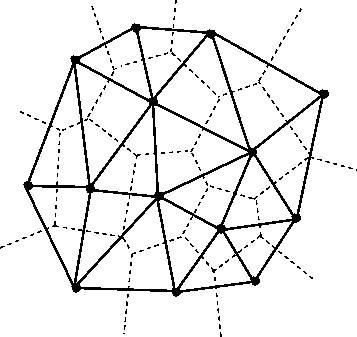
\includegraphics[width=4.5cm]{MyImages/delaugnay1.jpg} 
  & \hspace{2mm} &
  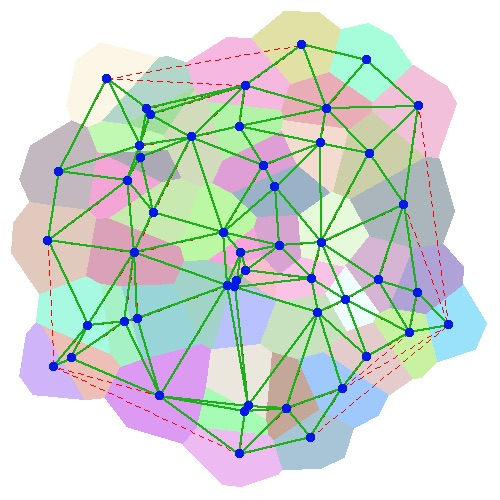
\includegraphics[width=4.5cm]{MyImages/delaugnay2.jpg}
\end{tabular}

 The Voronoy diagram is the dual of the Delaugnay tessellation.
\end{center}
\bigskip

\end{frame}



%----------------------------------------------
\begin{frame}
  \frametitle{Discontinuities and occlusion}
  \begin{itemize}
  \item It is possible to perform discontinuous regularization, where
    the smoothness term is disregarded when the surface is bended more
    than some threshold.
  \item Discontinuities are accompanied by occluded areas. If any
    point in an occluded area is matched it will be wrong. If not, the
    surface will be reconstructed more smooth than what it should.
  \end{itemize}

\begin{center}
  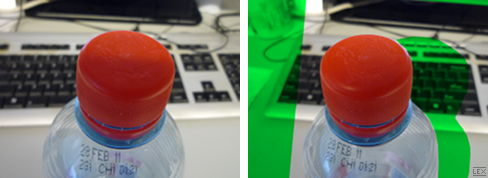
\includegraphics[width=8.0cm]{MyImages/3d-occlusion.jpg} 
\end{center}
\end{frame}




%----------------------------------------------
\begin{frame}
\frametitle{Methods for discontinuity detection etc}
\begin{itemize}
   \item Monitor matching strength or success rate. \\[3mm]
   \item Use of bipartite matching \\[3mm]
   \item Detecting large disparity gradients, application of
     discontinuous regularization / surface approximation. \\[3mm]
   \item Deletion of isolated feature matches. \\[3mm]
   \item Use of more advanced matching procedures like 
             {\em support matching}. Collect support to candidate
             solutions from all possible neighboring candidate solutions:
           $S({\bf p}_L^1, {\bf p}_R^1; \;\; 
                {\bf q}_L^2, {\bf q}_R^2)$
           The use of support functions is potentially strong, may
           facilitate fusion of semi-transparent surfaces, but may
           be computationally expensive.
  \end{itemize}
\end{frame}





%----------------------------------------------
\begin{frame}
  \frametitle{Support stereo}

The support $S$ of  $({\bf q}_L, {\bf q}_R)$ with disparity $d^q$
to  $({\bf p}_L, {\bf p}_R)$ with disparity $d^p$ should be: \\

 \begin{itemize}
  \item Decreasing in distance $r = |{\bf p}_L  - {\bf q}_L|$.
  \item Decreasing in disparity difference $\Delta = |d^p - d^q|$.
  \item Smooth, positive
  \end{itemize}
Example:
$$
  S = \frac{1}{r} \;  e^{- \lambda \Delta}
$$

Depending on the exact definition of $S$, highly efficient 
{\color{red}{Graph-cut}}-methods might be applied.
\end{frame}






%----------------------------------------------
\begin{frame}
\frametitle{Example}
{\tiny
The images in this and the next slides are from Scharstein, Szeliski:
{\em A taxonomy and Evaluation of Dense Two-Frame Stereo
  Correspondence Algorithms}, Int.Jour. of Comput.Vis. 47, 2002.
}

 \begin{center}
  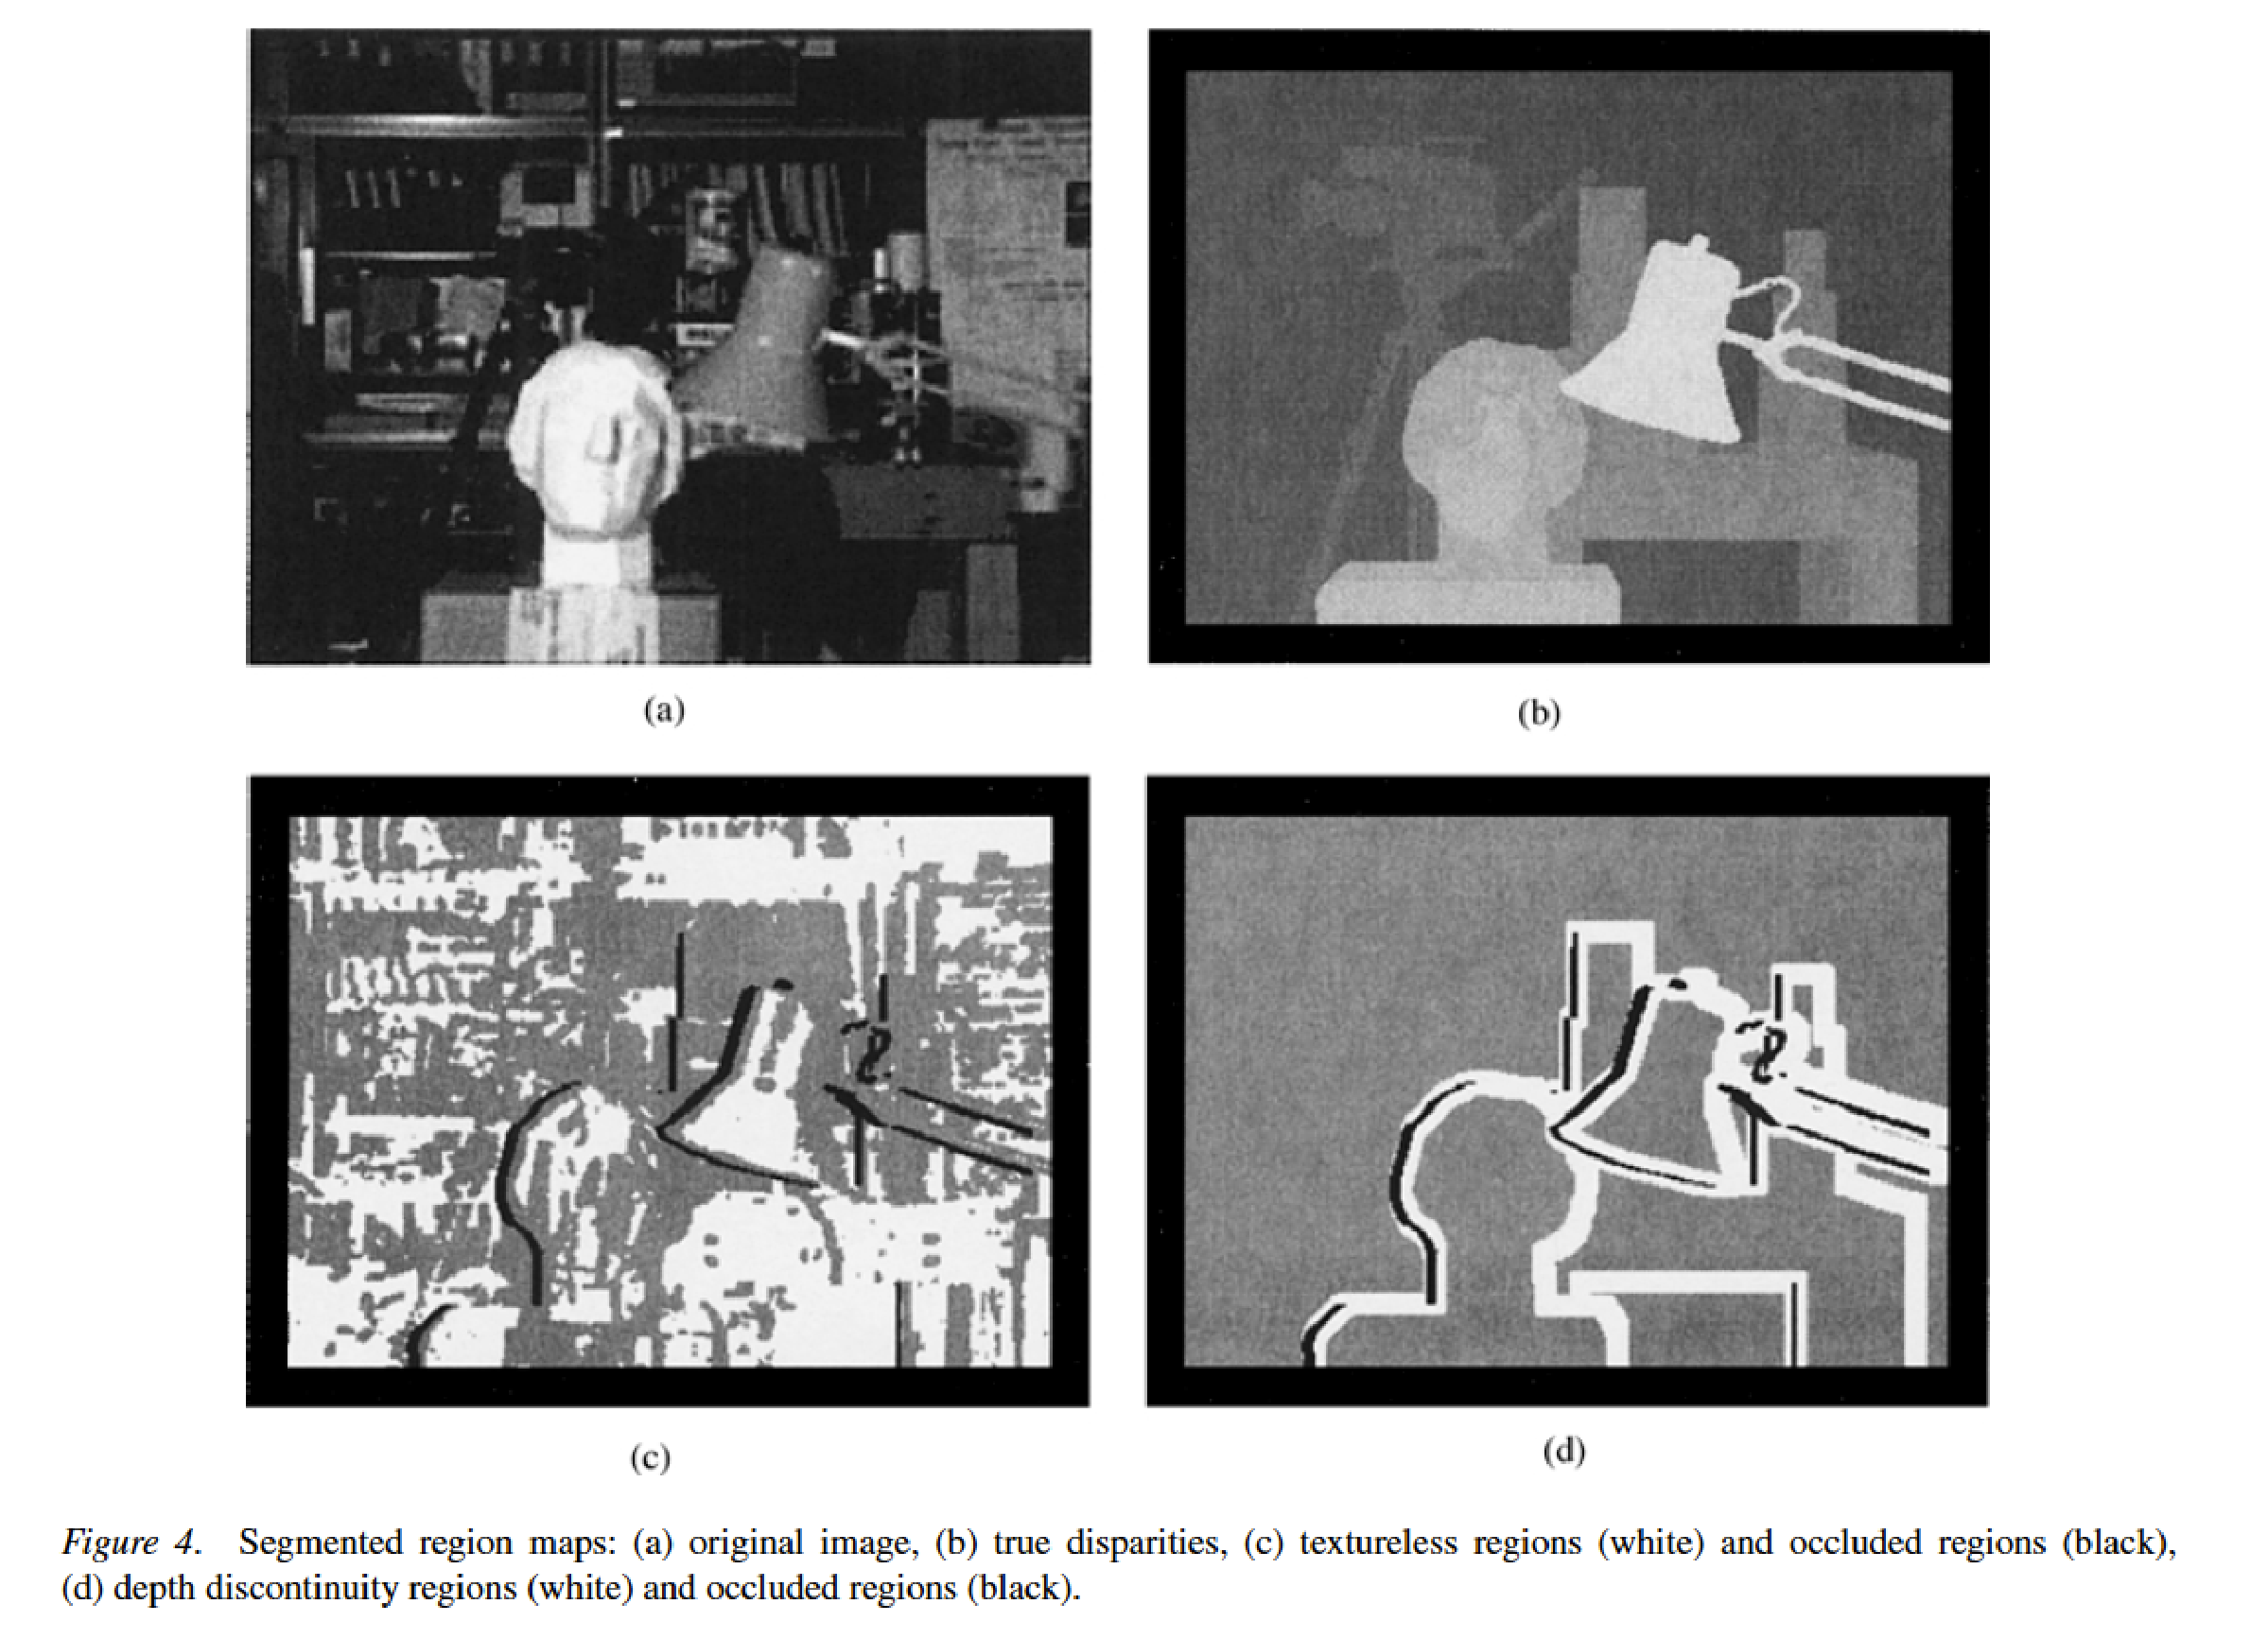
\includegraphics[width=8.0cm]{MyImages/ImStolen.pdf} 
\end{center}
\end{frame}



%----------------------------------------------
\begin{frame}
% \frametitle{Example}
 \begin{center}
  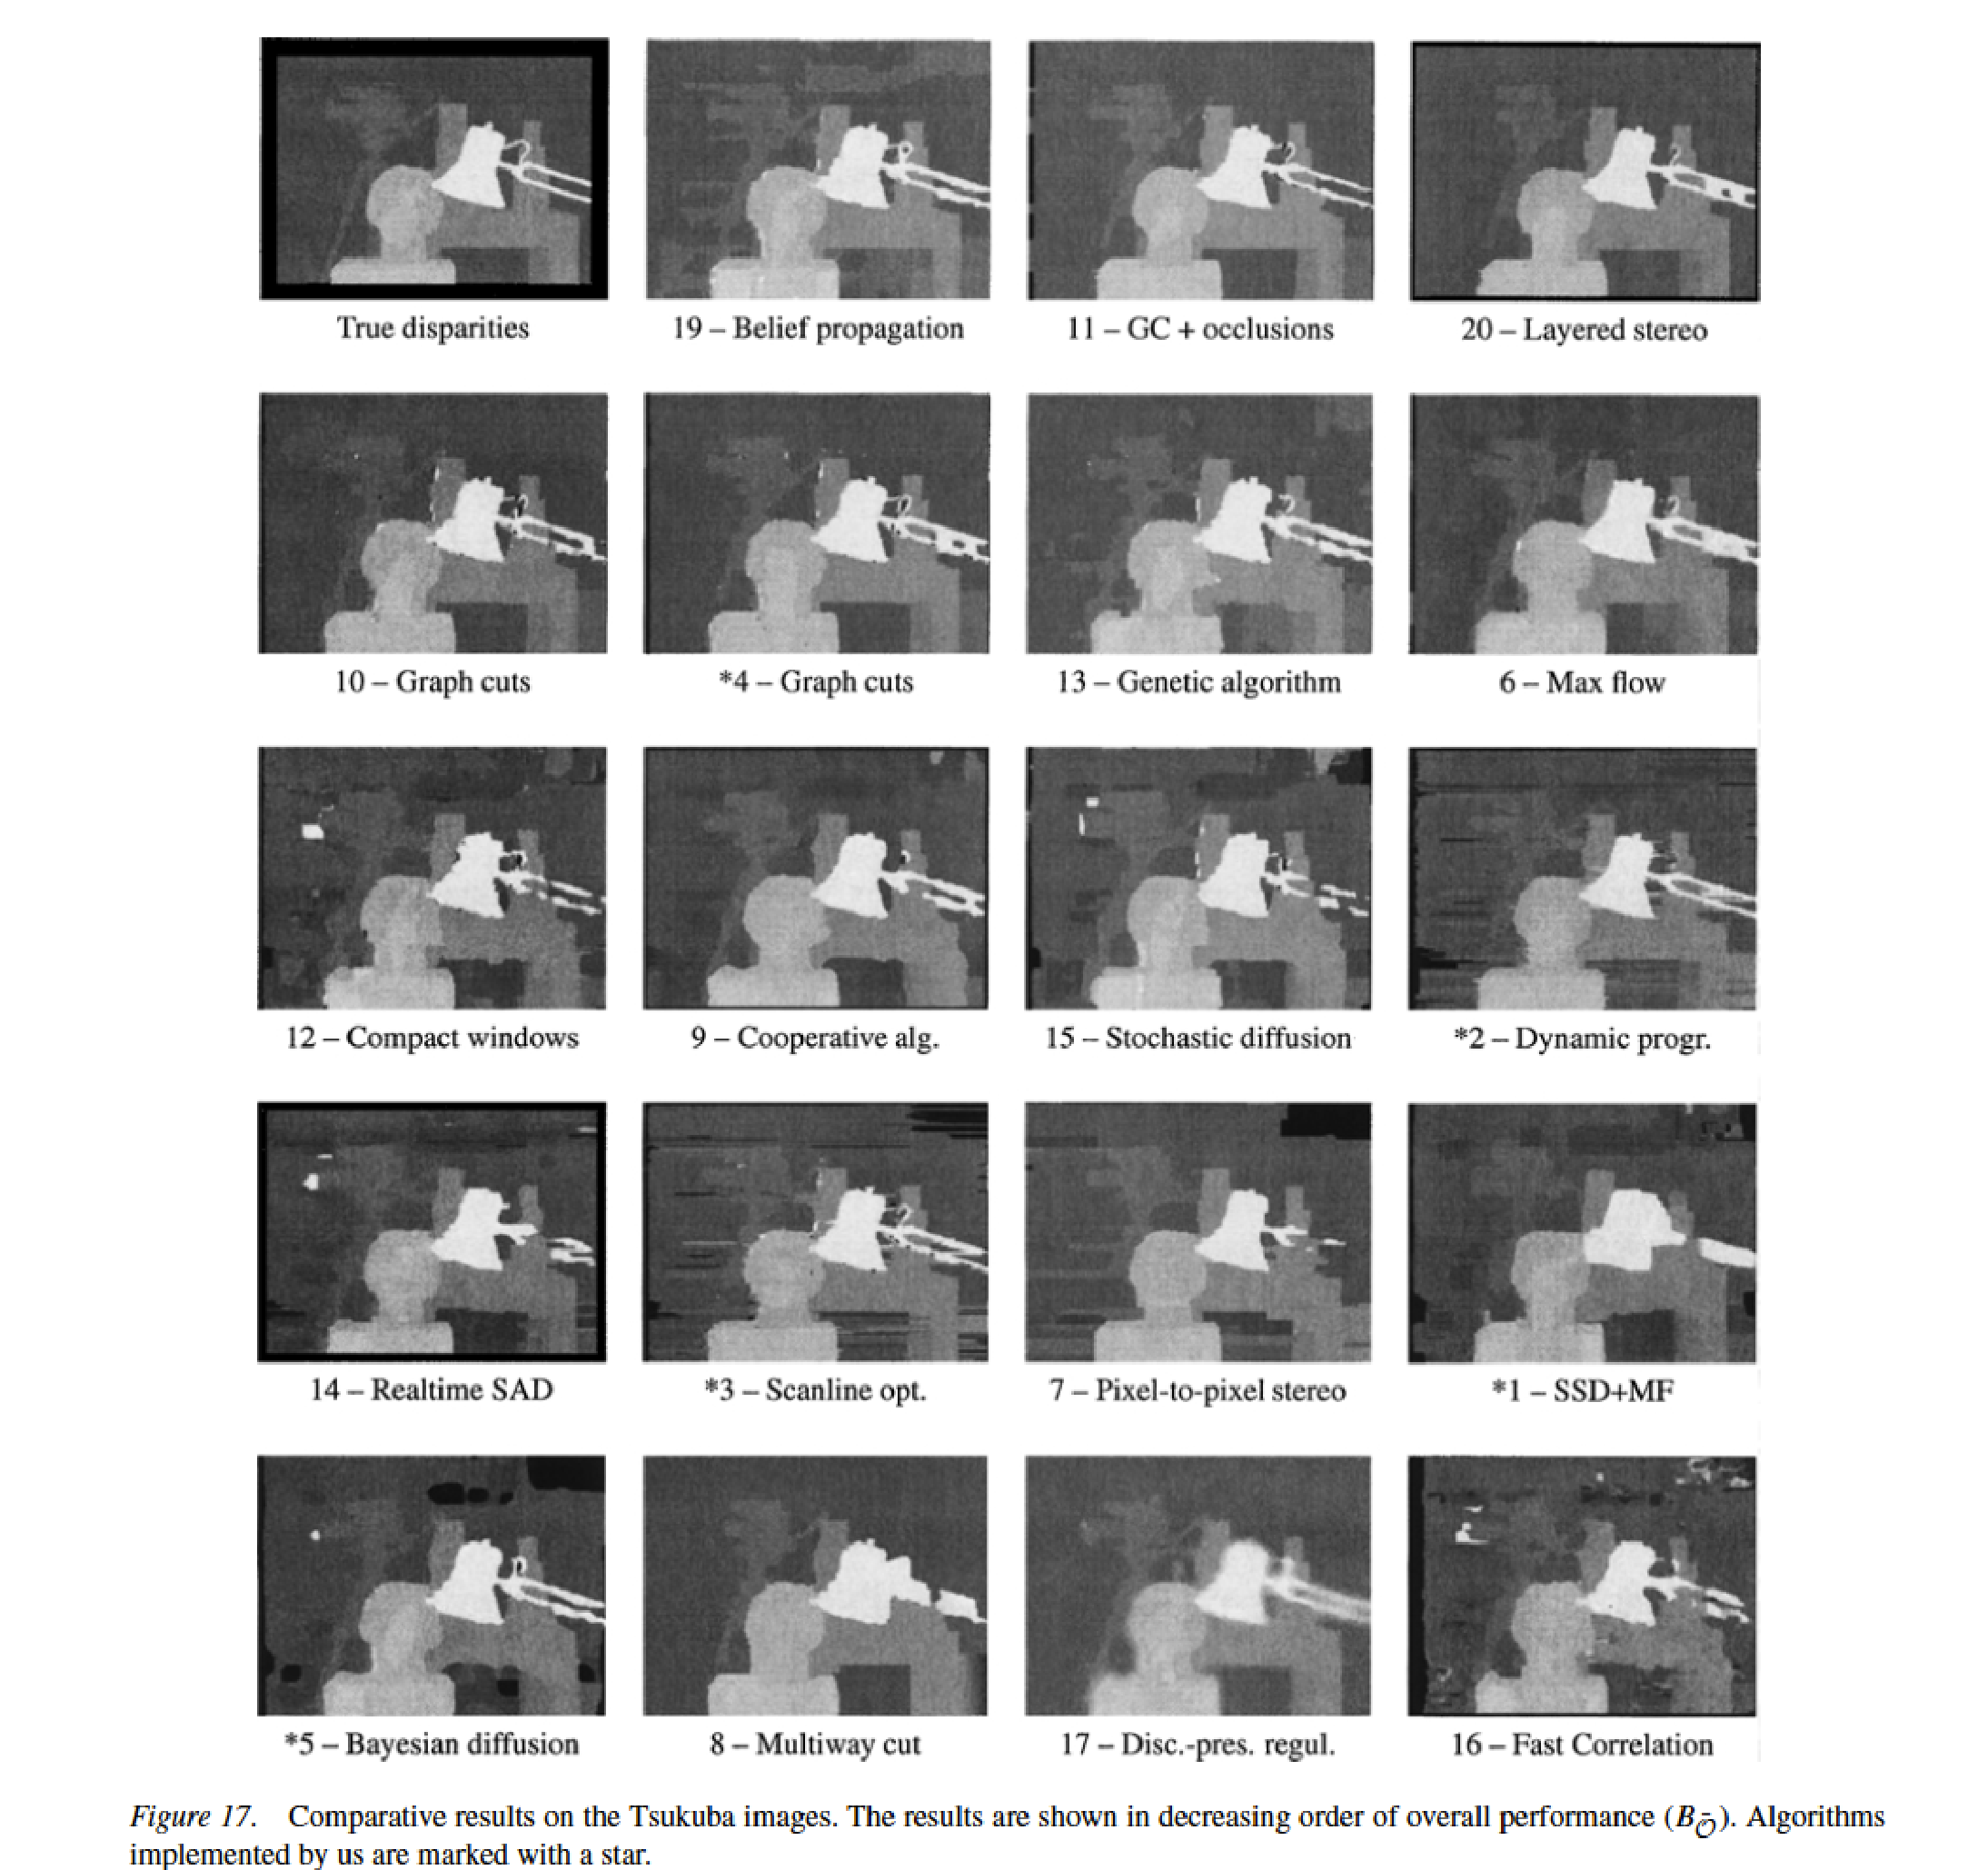
\includegraphics[width=9.0cm]{MyImages/ImStolen2.pdf} 
\end{center}
\end{frame}



%----------------------------------------------
\begin{frame}
  \frametitle{Other methods}
You may find many other approaches in the literature, eg.
a Dynamic-programming approach, See Forsyth and Ponce 2ed. 
Section 7.5.2.
%\bigskip

  \begin{center}
    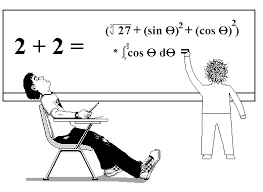
\includegraphics[width=0.5\textwidth]{MyImages/keepitsimple.png}
  \end{center}

For assignment 3, you are advised to do something simple that
you might get to work rather than more advanced methods.
\end{frame}




%----------------------------------------------
\begin{frame}
\frametitle{Where to find more information}
Most of the stuff today is found in [1] where parts are available in
copies at Absalon.  A comprehensive but not very readable treatment
may be found in [2] (the bible of 3DCV). [3] gives a good a readable
treatment. It is not mathematically deep, but contains many program
sketches. [4] is modern, very accessible but a bit superficial and 
focused on Python implementation.

  \begin{enumerate}
    \item Forsyth, Ponce: {\em Computer Vision - A modern approach},
      2.ed, Pearson 2012
    \item Hartley, Zisserman: {\em Multiple View Geometry in computer
        Vision}, 2.ed, Cambridge 2003
    \item Trucco, verri: {\em Introductory Techniques for 3-D Computer
        Vision}, Prentice Hall, 1998
    \item Solem: {\em Programming Computer Vision with Python},
      O'Reilly, 2012
   \end{enumerate}
\end{frame}






%----------------------------------------------
\begin{frame}
\frametitle{Outline of reconstruction procedure}
  \begin{enumerate}
   \item From interest point matches estimate fundamental matrix $F$
   \item From $F$ compute correspondences and camera matrices $C$ and $C'$
   \item From point correspondences and camera matrices compute 3D
     points. \\[3mm]
  \end{enumerate}

We will work our way backwards. Under way we will examine a set of
problems and solutions.  We will learn to solve homogeneous linear
equations $A {\bf x} = {\bf 0}$.   First however, we shall remember
the fundamental matrix equation.
\end{frame}





%----------------------------------------------
\begin{frame}
   \frametitle{Repetition: The fundamental matrix $F$}
   \begin{itemize}
      \item $F$ relates all point correspondences by $p_R^{\top} F p_L = 0$
     \item Given (sufficient) image point correspondences, the
       fundamental matrix $F$ may be estimated
       using linear algebra. 
     \item $F$ has only 7 degrees of freedom (not 9) because it is
       defined up to scaling only, and because $\det (F) = 0$.
     \item Linear estimation of $F$   is easy, but not accurate. In
       practice a non-linear post-optimization is needed.
      \item Given $F$, the stereo correspondence problem is reduced
        to a one-dimensional search along the epipolar lines. 
      \item Given projections $(x,y)$ of known 3D points $(X,Y,Z)$,
        the calibration matrix $K$ may be estimates using linear algebra.
      \item Given $F$, $K$ and $K'$, reconstructions of 3D points is
        possible (using linear algebra) from image point correspondences.
   \end{itemize}
\end{frame}



%----------------------------------------------
\begin{frame}
\frametitle{Proof of $x_R^{\top}Fx_L = 0$}
\begin{center}
      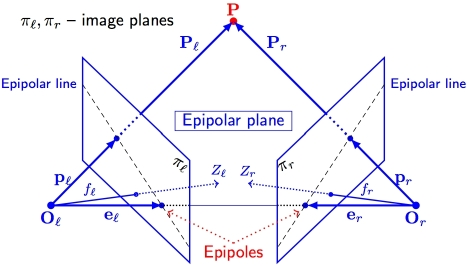
\includegraphics[width=0.7\textwidth]{MyImages/epipolarGeom.jpg}
\end{center}
We have that the camera coordinate systems are related by:
\begin{displaymath}
   {\bf P}_R = R ( {\bf P}_L - {\bf T})
\end{displaymath}

\begin{definition}
  The coplanarity condition:  
  ${\bf P}_L$, ${\bf T}$, and 
  ${\bf P}_L - {\bf T}$ are all in the epipolar plane. Then, also
   $R^{\top}{\bf P}_R$  is within the plane.
\end{definition}

\end{frame}



%----------------------------------------------
\begin{frame}
\frametitle{The cross-product}
The cross-product between two vectors ${\bf a}$ and ${\bf b}$ is a
vector that is perpendicular to both:

\begin{displaymath}
   {\bf a} \times {\bf b} \;=\; 
   \left ( 
   \begin{array}{c}
   -a_3 b_2 + a_2 b_3 \\ a_3 b_1 - a_1 b_3 \\ -a_2 b_1 + a_1 b_2
    \end{array}
    \right )
    \;=\; S {\bf b}
\end{displaymath}
where 
\begin{displaymath}
   S \;=\; [a]_x \;=\; \left [
     \begin{array}{c c c}
        0    & - a_3 & a_2  \\ 
        a_3 &    0    & -a_1 \\
      -a_2 &  a_1   &  0
     \end{array}
   \right ]
\end{displaymath}

$\mbox{}$ \\[2mm]
We see that $S$ is an anti-symmetric and rank deficient matrix. $S$
has rank 2.
\end{frame}



%----------------------------------------------
\begin{frame}
 \frametitle{Proof cont. 2}
Because  ${\bf P}_L$, ${\bf T}$, and ${\bf P}_L - {\bf T}$ all are in
the epipolar plane we can write:
\begin{eqnarray*}
 0 & = &   ({\bf P}_L - {\bf T}) ^{\top} {\bf T} \times {\bf P}_L \\[2mm]
    & = &  (R^{\top}{\bf P}_R) ^{\top}{\bf T} \times {\bf P}_L \\[2mm]
    & = &  (R^{\top}{\bf P}_R) ^{\top} S {\bf P}_L\\[2mm]
    & = & {\bf P}_R^{\top} R S {\bf P}_L \\[2mm]
    & = & {\bf P}_R^{\top} E {\bf P}_L \\[2mm]
\end{eqnarray*}
where we have used that ${\bf P}_R = R ( {\bf P}_L - {\bf T})$ and 
$E = RS$.  

Since $\mbox{rank}(S) = 2$, $\mbox{rank}(E) = 2$. 
\end{frame}



%----------------------------------------------
\begin{frame}
\frametitle{The fundamental matrix equation once more}
We have now established the Essential matrix equation 
${\bf P}_R^{\top} E {\bf P}_L = 0$. To get to the fundamental matrix
equation we remember  the relation between the camera- and the image
coordinate systems:

\begin{displaymath}
     K \;=\;
     \begin{pmatrix}
       \alpha & s & u_0\\
       0 & \beta & v_0\\
       0 & 0 & 1
     \end{pmatrix}
\end{displaymath}

Using ${\bf p}_L = K_L {\bf P}_L$ and ${\bf p}_R = K_R {\bf P}_R$ 
and defining 
\begin{displaymath}
  F \;=\; K_R^{-\top} E K_L^{-1}
\end{displaymath}
we finally get:
\begin{displaymath}
  {\bf p}_R^{\top} F {\bf p}_L \;=\; 0
\end{displaymath}


\end{frame}



%----------------------------------------------
\begin{frame}
 \frametitle{3-Camera stereo}

The use of 3 cameras in stereo vision, and assuming all fundamental
matrices known, makes the correspondence analysis more easy and
robust. 


\begin{center}
      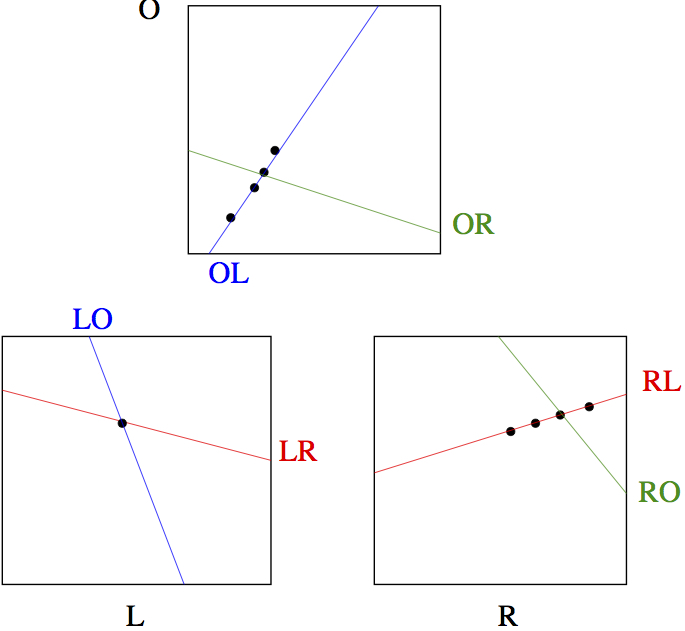
\includegraphics[width=0.6\textwidth]{FIGURES/kamera3.jpg}
\end{center}

\end{frame}



%----------------------------------------------
\begin{frame}
 \frametitle{The epipoles}
Remember the fundamental matrix equation:
\begin{displaymath}
  (x_R, y_R, 1)  F 
  \left (
  \begin{array}{c} x_L \\ y_L \\ 1 \end{array}
  \right )
  \;\; = \;\; 0
\end{displaymath}
The left epipole ${\bf e_L}$ is the $(x_L, y_L)$ that makes the equation
true for all $(x_R, y_R)$.  Thus:
\begin{displaymath}
   F {\bf e_L}  = 0  
  \hspace{1cm} \mbox{and} \hspace{1cm}
  {\bf e_R} F = 0
\end{displaymath}
The epipoles are the left and right kernel of $F$.
\end{frame}




% ------------------------------------------
\begin{frame}
\frametitle{Singular value decomposition (svd)}
The svd of a $m \times n$ matrix $A$ is a factorization:
\begin{displaymath}
  A \;=\; U D V^{\top}
\end{displaymath}
where $U$ is $m \times n$ and $U U^{\top} = I$, $D$ is a diagonal 
$n \times n$ matrix with non-negative singular values, and $V$ is a
$n \times n$ unitary matrix $V V^{\top} =  V^{\top} V = I$. \\[4mm]

We are not interested in the trivial solution ${\bf x = 0}$ but rather
all solution lying in the {\color{blue}{Null-space}} of the matrix
$A$. \\[4mm]

The singular values in the diagonal matrix $D$ specifies the
{\color{blue}{energy}} contained in each of the dimensions. Usually, these are
sorted in decreasing order. \\[4mm]

Often, due to noise all singular values $\sigma_i > 0$.  If we know
that $A$ should be singular may find the closest such matrix by
zeroing out the smallest singular value. 
\end{frame}




%----------------------------------------------
\begin{frame}[fragile]
\frametitle{Solving $A {\bf x} = {\bf 0}$}

From the SVD-decomposition:
\begin{displaymath}
  A \;=\; U D V^{\top}
\end{displaymath}

we get the solution to $A {\bf x} = {\bf 0}$ as the last column of
$V$. \\[4mm]

In MATLAB: \\
\texttt{
[U,D,V] = svd(F); eL = V(:,end); eR = U(:,end);
} \\[4mm]

Since the fundamental matrix $F$ is singular, the smallest singular value
will be zero.  Thus, the solution to 
$F {\bf e_L}  = U D V^{\top} {\bf e_L} = 0$
will be the last column of $V$ corresponding to the null singular value.\\[4mm]

Similarly, ${\bf e_R}$ is the column of $U$ corresponding to the null
singular value.
\end{frame}



%----------------------------------------------
\begin{frame}
\frametitle{Repetition: The camera matrix}
Please recall the definition of the camera matrix:
\begin{displaymath}
      M =  K \left[ R \,\, {\bf t}\right]
\end{displaymath}
and the projection written out:
\begin{displaymath}
   w
   \begin{bmatrix}
     x\\y\\1
   \end{bmatrix}
   = \udesc{{\bf K}}{
     \begin{pmatrix}
       f_x & 0 & u_0\\
       0 & f_y & v_0\\
       0 & 0 & 1
     \end{pmatrix}}
   \udesc{\left[{\bf R}\,\, {\bf t}\right]}{
     \begin{pmatrix}
       r_{11} & r_{12} & r_{13} & t_x\\
       r_{21} & r_{22} & r_{23} & t_y\\
       r_{31} & r_{32} & r_{33} & t_z\\
     \end{pmatrix}}
   \begin{pmatrix}
     X\\Y\\Z\\1
   \end{pmatrix}
\end{displaymath}
or
\begin{displaymath}
   w
   \begin{bmatrix}
     x\\y\\1
   \end{bmatrix}
   =
     \begin{pmatrix}
       {\bf m}^1 \\
       {\bf m}^2 \\
       {\bf m}^3 \\
     \end{pmatrix}
   \begin{pmatrix}
     X\\Y\\Z\\1
   \end{pmatrix}
\end{displaymath}
where ${\bf m}^i$ is the $i$'th row of the camera matrix. 
\end{frame}


%----------------------------------------------
\begin{frame}
\frametitle{Linear triangulation}
Let $U = (X, Y, Z, 1)^{\top}$.  For the first coordinate in the left camera we have:
\begin{displaymath}
 x^L  = \frac{{\bf m}_L^1U}{{\bf m}_L^3U}
\end{displaymath}
and similar for the $y$-coordinate and the right camera.  Multiplying
by the denominator we get:
\begin{eqnarray*}
   {\bf m}_L^3 x_L  U & = & {\bf m}_L^1 U \\
   {\bf m}_L^3 y_L  U & = & {\bf m}_L^2 U \\
   {\bf m}_R^3 x_R U & = & {\bf m}_R^1 U \\
   {\bf m}_R^3 y_R U & = & {\bf m}_R^2 U 
\end{eqnarray*}
Subtracting the right side and putting $U$ outside a parentesis we get
the homogeneous equation $A U = 0$, where:
\begin{displaymath}
  A  = \left (
    \begin{array}{c}
   {\bf m}_L^3 x_L   - {\bf m}_L^1 \\
   {\bf m}_L^3 y_L   - {\bf m}_L^2 \\
   {\bf m}_R^3 x_R  - {\bf m}_R^1 \\
   {\bf m}_R^3 y_R  - {\bf m}_R^2 
      \end{array}
    \right )
\end{displaymath}
\end{frame}




%----------------------------------------------
\begin{frame}
\frametitle{Algebraic reconstruction is not optimal}
\begin{itemize}
\item  The solution above was achieved from solving the projection
  equations assuming that the points $(x_L, y_L)$ and $(x_R, y_R)$
  both have infinite precision.  It is not explicit and clear what is
  the properties of the solution (what is minimized). \\[4mm]
\item A better formulation of the problem is when the error measure
  (to be minimized) is in terms of image distances (pixels). \\[4mm]
\item We search the the 3D point $U$ that is projected on points 
  $\hat{x}_L$ and $\hat{x}_R$ such that these points are close to the
  matched points  $x_L$ and $x_R$ 
\end{itemize}
\end{frame}




%----------------------------------------------
\begin{frame}
\frametitle{The reprojection error}
  \begin{center}
    \includegraphics[width=0.85\textwidth]{FIGURES/reprojectionerror.png}
  \end{center}

The reprojection error is the sum of distances:
\begin{displaymath}
    E_{\mbox{rep}}  = dist(x_L, \hat{x}_L) \;+\; dist(x_R, \hat{x}_R) \hspace{3mm}
    \mbox{subject to $\hat{x}_R^{\top} F \hat{x}_L = 0$}
\end{displaymath}
where $F$ is the fundamental matrix. This formulation above is not
linear but can be shown to end up in a root-finding of a polynomium of
degree 6. 
\end{frame}




%----------------------------------------------
\begin{frame}
\frametitle{Algebraic solution versus Gold standard}
\begin{itemize}
\item The Gold standard approach always minimizes something that we
  can measure in the image plane.  \\[4mm]
\item The Gold standard approach is the right way to solve the problem 
  but is typically not linear. Thus it is neither easy nor fast. \\[4mm]
\item Often Algebraic linear approaches are used as initial values for
  non-linear optimization approaches using the Gold standard.
\end{itemize}
\end{frame}




%----------------------------------------------
\begin{frame}
\frametitle{Estimation of the camera matrix \\ using a calibration
  object}

If you have a 3D calibration object with known relative 3D positions
$U = (X, Y, Z)^{\top}$ and their projected image coordinates we may
calibrate the camera.

   \begin{center}
      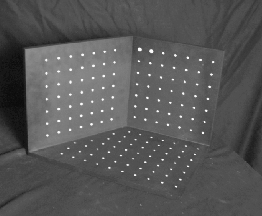
\includegraphics[width=0.50\textwidth]{IMAGES/calibrationobject}
  \end{center}
\end{frame}




%----------------------------------------------
\begin{frame}
\frametitle{Camera calibration 1}
In Camera calibration the task first is to recover the 12 unknowns ${\bf m}_{ij}$
in the camera calibration matrix.  Here we use simple linear algebra. We
have: 
\begin{eqnarray*}
   x {\bf m}_3 U & = & {\bf m}_1 U \\
   y {\bf m}_3 U & = & {\bf m}_2 U 
\end{eqnarray*}

Let ${\bf m} = (m_{11}, \ldots , m_{14} , \ldots, m_{34})^{\top}$ be the
vector of the 12 unknowns.  Isolating these in the equations above
lead to: $A {\bf m} = 0$, where:

{\tiny
\begin{displaymath}
 A \;=\; \left [
    \begin{array}{cccccccccccc}
       X_1 & Y_1 & Z_1 & 1 & 0 & 0 & 0 & 0 & -x_1X_1 & -x_1Y_1 & -x_1Z_1 & - x_1 \\
       0 & 0 & 0 & 0 & X_1 & Y_1 & Z_1 & 1 & -y_1X_1 & -y_1Y_1 & -y_1Z_1 & - y_1 \\
       X_2 & Y_2 & Z_2 & 1 & 0 & 0 & 0 & 0 & -x_2X_2 & -x_2Y_2 & -x_2Z_2 & - x_2 \\
       0 & 0 & 0 & 0 & X_2 & Y_2 & Z_2 & 1 & -y_2X_2 & -y_2Y_2 & -y_2Z_2 & - y_2 \\
       \vdots & \vdots & \vdots & \vdots & \vdots & \vdots & 
       \vdots & \vdots & \vdots & \vdots & \vdots & \vdots \\
       X_N & Y_N & Z_N & 1 & 0 & 0 & 0 & 0 & -x_NX_N & -x_NY_N & -x_NZ_N & - x_N \\
       0 & 0 & 0 & 0 & X_N & Y_N & Z_N & 1 & -y_NX_N & -y_NY_N & -y_NZ_N & - y_N 
   \end{array}
   \right ]
\end{displaymath}
}
\end{frame}



%----------------------------------------------
\begin{frame}
\frametitle{Camera calibration 2}
Since $A {\bf m} = 0$ is homogeneous, it has rank 11, and the solution may
be found using a SVD-factorization as described before. \\[4mm]

Using the definition of the camera calibration matrix, It is possible 
(given ${\bf m}$), to solve for the focal lengths $f_x$ and $f_y$, the
principal point $(u_0, v_0)$, the translation vector $(t_x, t_y, t_z)$
and the rotation matrix $R$. \\[4mm]

There are several approaches to extracting these parmeters. Please
check the literature (see slide 12).  
\end{frame}



%----------------------------------------------
\begin{frame}
\frametitle{Estimation of the camera matrix from $F$}
If you do not have a 3D calibration object the relative calibration
matrix of the second camera may be estimated from the fundamental
matrix $F$. \\[4mm]

Assume that the camera matrix of the first camera may be chosen as 
{\color{red}{$K [I | 0]$}}, ie. $R$ is fixed to the identity matrix and the
translation vector to the zero-vector. Then we can compute the second
camera matrix C from $F$ by: 

\begin{displaymath}
   C \;=\;  \left [ ([e_R]_x  F) \;\; | \;\; e_R \right ]
\end{displaymath}

where $e_R$ is the right epipole, computed as the solution to 
$e_RF = 0$ and where $[e]_x$ is the $3 \times 3$ antisymmetric
matrix constructed from the vector $e$ (please see slide 15 on the
cross-product). \\[4mm] 

You may find the proof of this in Hartley and Zisserman [2]. 
\end{frame}



%----------------------------------------------
\begin{frame}
\frametitle{Estimation of the fundamental matrix F}
$F$ is defined by
{\color{red}{$x_R' F x_L= 0$}} 
% $x_R' F x_L= 0$
where  $x_R'$ and $x_L$ are corresponding image points in homogeneous 
coordinates. \\[4mm] 

$F$ has 9 elements, but only 7 degrees of freedom. If we have
at least 8 correspondences (hopefully more, but not necessarily
hundreds) we may estime $F$ using the 
{\color{blue}{8-point algorithm}} \\[5mm]

The basic 8-point alg.\ may be improved by normalization and by
making it robust to false correspondences (using 
{\color{blue}{RANSAC}}).  Often in practice it is used for initializing
a non-linear optimization estimation.  Thus it is necessary, but not
always sufficient. 
\end{frame}



%----------------------------------------------
\begin{frame}
\frametitle{The 8-point algorithm 1}
Writing out the definition and isolating the 9 elements of $F$ as a
vector ${\bf f}$ we get for $n$ correspondences:

\begin{displaymath}
 A {\bf f} \;=\; \left [
    \begin{array}{ccccccccc}
       x_R^1 x_L^1 & x_R^1 y_L^1 & x_R^1 & y_R^1 x_L^1 & y_R^1 y_L^1 & y_R^1 & x_L^1 & y_L^1 & 1 \\
       \vdots & \vdots & \vdots & \vdots & \vdots & \vdots &  \vdots & \vdots \\
       x_R^n x_L^n & x_R^n y_L^n & x_R^n & y_R^n x_L^n & y_R^n y_L^n & y_R^n & x_L^n & y_L^n & 1 
   \end{array}
   \right ]
    {\bf f} \;\;=\;\; {\bf 0} 
\end{displaymath}

$\mbox{}$\\[3mm]
As before we solve this homogeneous equation by the last column of the
matrix $V$ in a SVD-decomposition $A = U D V^{\top}$ of $A$. From
${\bf f}$ we construct the matrix $\tilde{F}$.
\end{frame}



%----------------------------------------------
\begin{frame}
\frametitle{The 8-point algorithm 2}
The fundamental matrix must have rank 2.  In general the estimated
matrix $\tilde{F}$ have rank 3.  To find the rank-2 matrix most
similar to $\tilde{F}$, we make a SVD of this:

\begin{displaymath}
    \tilde{F} \;=\; U D V^{\top}
\end{displaymath}

Then we set the smallest of the singular values in $D$ to zero and
multiply with $U$ and $V^{\top}$. \\[5mm]

The resulting matrix $\hat{F}$ will have 7 degrees of freedom
(and rank 2).
\end{frame}





%----------------------------------------------
\begin{frame}
\frametitle{Normalization}
Image coordinates run from $0$ to some large number and appears in
$A$ in products, alone, and together with the constant $1$. Rows with
large coordinate value will contribute much more to the solution. \\[3mm]

To reduce the effect and improve numerical stability we subtract the
mean coordinate value and divide by $\sigma/\sqrt{2}$ where $\sigma$
is the standard deviation of the coordinate value.  This linear
operation may be expressed as a preprocessing:
\begin{displaymath}
   \hat{{\bf x}_L^i} = T_L  {\bf x}_L^i 
   \hspace{4mm} \mbox{and}   \hspace{4mm}
   \hat{{\bf x}_R^i} = T_R  {\bf x}_R^i 
\end{displaymath}

After estimating the fundamental matrix this has to be denormalized
accordingly: 
\begin{displaymath}
   F = T_R^{\top} \hat{F} T_L
\end{displaymath}
 
\end{frame}




%----------------------------------------------
\begin{frame}
\frametitle{RANSAC 1}
Frequently even the best matching algorithm makes errors. Just a
single false match may ruin (all of) the estimation procedures treated
so far.  We need to be robust to false matches (outliers). \\[4mm]

{\color{blue}{Random Sample Consensus}} is one of the most celebrated
algorithms for robust estimation.  RANSAC may tolerate up to 50\% and
even more outliers and still produce the right result. \\[4mm]

RANSAC builds on random sampling of exactly as many data as there is
parameters to estimate and assumes a procedure for such estimation. \\[4mm]

We will go through the details of RANSAC next time (Monday Januar 12).

\end{frame}




%----------------------------------------------
\begin{frame}
\frametitle{Evaluation of $F$}
Assume that we have estimated the fundamental matrix as well as
possible. Then we may draw the epipolar lines on the image to evaluate 
informally. Often we get something like the bottom row:

  \begin{center}
    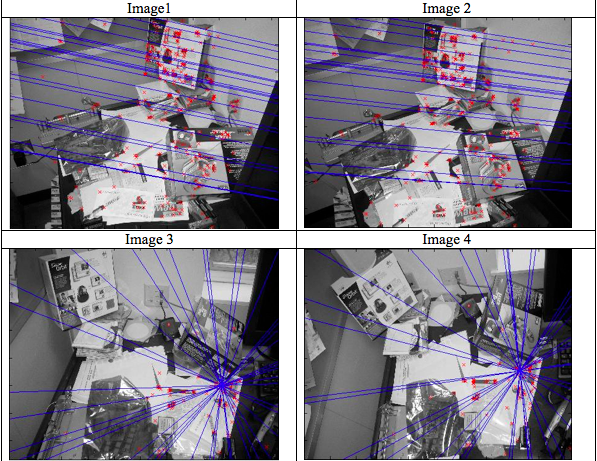
\includegraphics[width=0.55\textwidth]{MyImages/epipolar.png}
  \end{center}
  
Problem: Estimation of $F$ is numerically unstable and using an
algebraic approach is often not sufficient.
\end{frame}



%----------------------------------------------
\begin{frame}
\frametitle{Non-linear estimation of $F$}
  \begin{center}
    \includegraphics[width=0.65\textwidth]{FIGURES/reprojectionerror.png}
  \end{center}

We want to minimize the reprojection error:
\begin{displaymath}
    E_{\mbox{rep}}  = dist(x_L, \hat{x}_L) \;+\; dist(x_R, \hat{x}_R) \hspace{3mm}
    \mbox{subject to $\hat{x}_R^{\top} F \hat{x}_L = 0$}
\end{displaymath}

Thus we both want to find $F$ and the ``true'' projections $\hat{x}_L$
and $\hat{x}_R$ simultaneously. This is a non-linear formulation and
requires non-linear numerical optimization methods to selve.

\end{frame}






%----------------------------------------------
\begin{frame}
\frametitle{2D Homography}
  \begin{itemize}
   \item The relationship between two 2D perspective projections of a 3D
     planar scene surface is called an \myemph{homography}:
     $$
     \begin{bmatrix}
       w x\\w y\\w
     \end{bmatrix}
     =
     \begin{pmatrix}
       h_{11} & h_{12} & h_{13} \\
       h_{21} & h_{22} & h_{23} \\
       h_{31} & h_{32} & h_{33} 
     \end{pmatrix}
     \begin{bmatrix}
       x'\\y'\\1\\
     \end{bmatrix}
     =
     H \cdot {\bf x}'
     $$
   \item Homographies are used for stitching, pedestrian detection,
     geo-referencing etc. 
   \item Homographies are estimated exactly as fundamental matrices
     but have (in general) full rank.
  \end{itemize}
\end{frame}





%----------------------------------------------
\begin{frame}
  An homography can accurately describe the transformation between two
  perspectively projected images. \\[3mm]

  \begin{center}
    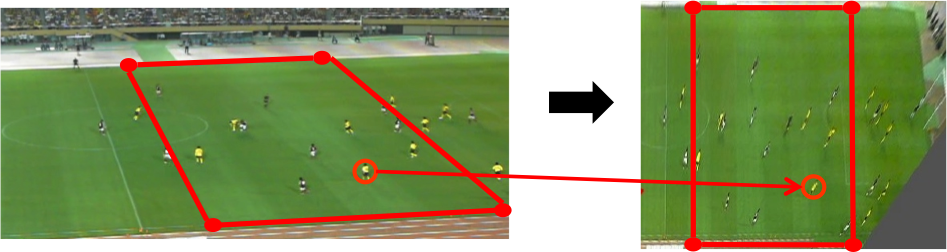
\includegraphics[width=0.95\textwidth]{MyImages/soccer_homography.png}
  \end{center}
  
  You are now be able to make a program showing if there was a goal or not.
\end{frame}




%----------------------------------------------
\begin{frame}
   \begin{center}
    
\includegraphics[width=\textwidth]{IMAGES/tired}
  \end{center}
\end{frame}



\end{document}

